\section{Sobre Usina de Salto Osório}

A Usina Hidrelétrica de Salto Osório localiza-se a $19,5~km$ da cidade de Quedas
do Iguaçu, estado do Paraná, sendo alimentada pelo Rio Iguaçu. É uma usina ``a
fio d'água'', que conta com $6$ turbinas em linha, do tipo Francis e tem uma potência
instalada de $1078~MW$.

Sua construção foi concluída em $1979$, sendo atulamente operada pela companhia
Tractebel Energia que é controlada pelo grupo franco-belga ENGIE. A operação da
usina conta com um total de $40$ funcionários na sua atividade-fim.

%TODO Incluir fotos da usina

\begin{figure}[h!]
\centering
	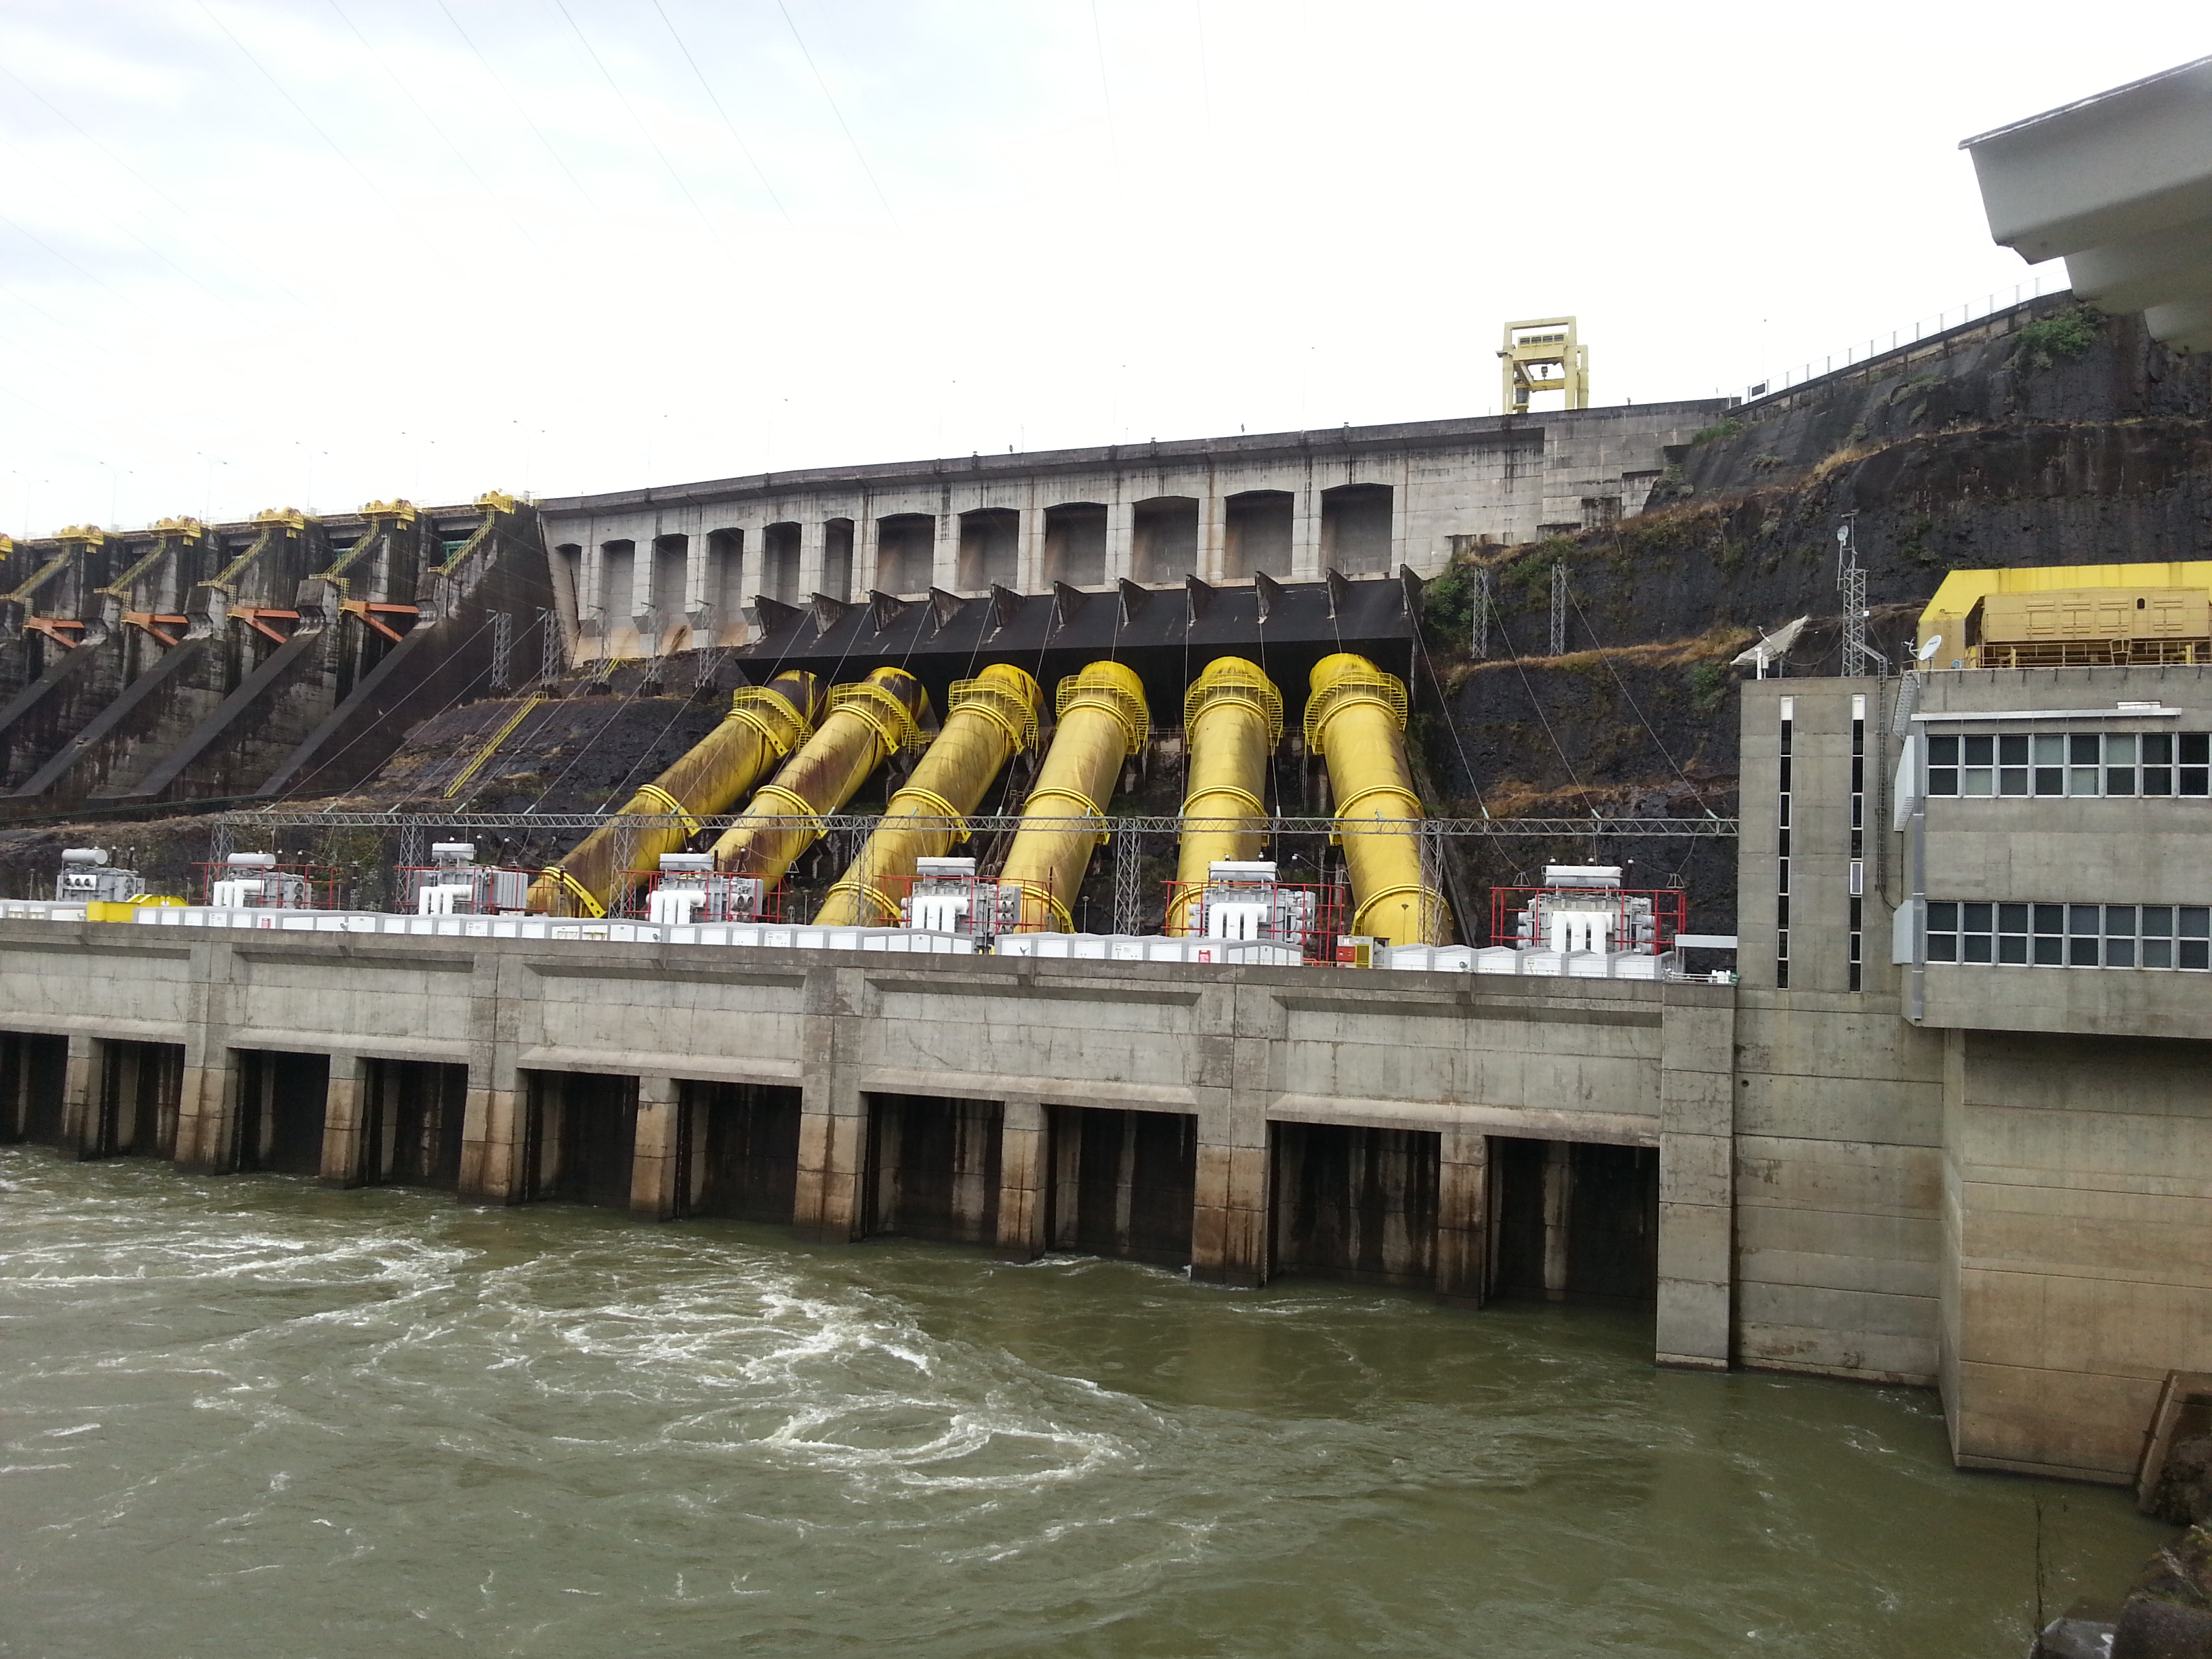
\includegraphics[width=0.9\columnwidth]{figs/usina_01}
	\caption{Vista da portaria da Usina Hidrelétrica de Salto Osório}
	\label{fig::usina_01}
\end{figure}

Para chegar à usina, a equipe viajou até Foz do Iguaçu, Paraná, desembarcando no
aeroporto de Foz do Iguaçu/Cataratas (IGU). Os equipamentos foram enviados em
uma caixa fechada, pesando aproximadamente $100~kg$, via TAM Cargo com
antecedência de $3~dias$, para ser retirada no mesmo aeroporto. Para transporte
dos passageiros e da caixa, com conforto e segurança, optou-se pelo aluguel de
uma caminhonete modelo Chevrolet S$10$. Pela proximidade da usina e
infra-estrutura da cidade, a equipe hospedou-se em Quedas do Iguaçu,
que fica localizada a uma distância de $256~km$ da cidade de Foz do Iguaçu e
$19,5~km$ da usina de Salto Osório.

O complexo da usina hidrelétrica conta com $6$ turbinas do tipo Francis, um
prédio administrativo, uma subestação de $230~kV$ e dois vertedouros. O veículo
da equipe, com os equipamentos, pôde ser estacionado próximo do vão do stoplog
para a instrumentaçào da Viga Pescadora. A área de acesso aos stoplogs é
equipada com uma ponte rolante que percorre toda a extensão da áera, permitindo
a manipulação da Viga Pescadora em todos os stoplogs. 

\begin{figure}[h!]
\centering
	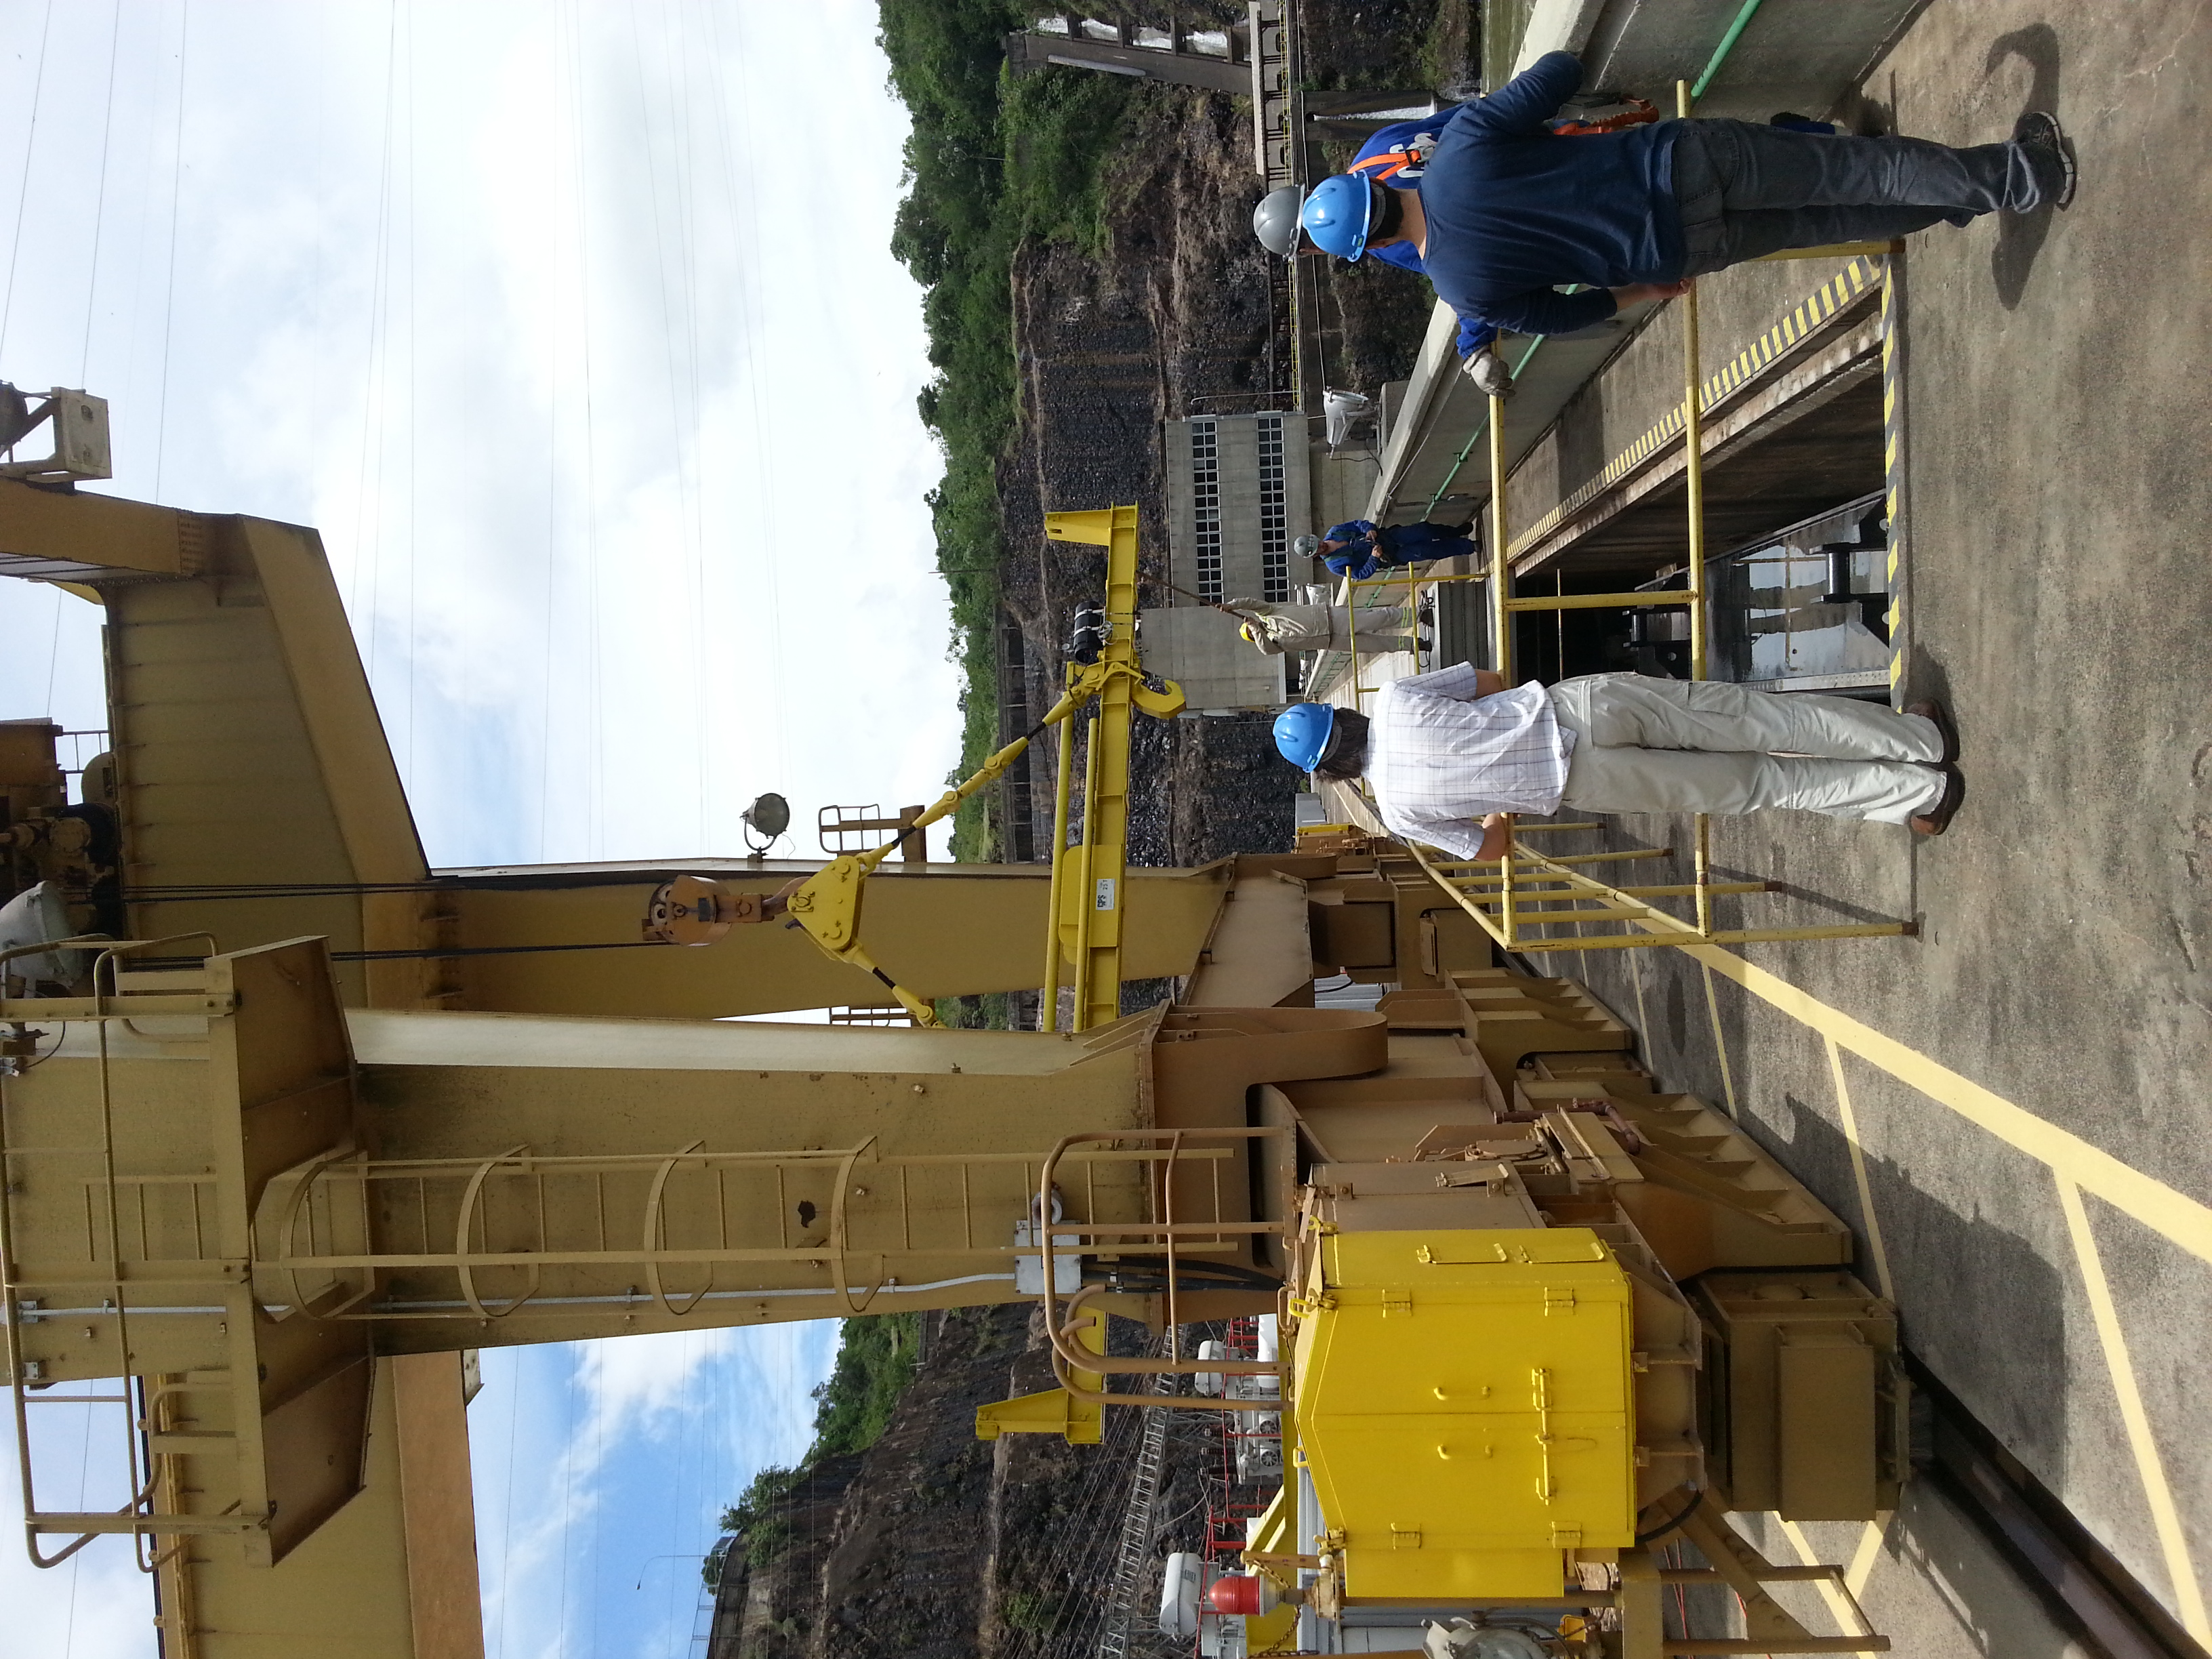
\includegraphics[width=0.9\columnwidth, angle=270]{figs/ponte_e_viga}
	\caption{Pórtico Rolante suspendendo Viga Pescadora}
	\label{fig::ponte_e_viga}
\end{figure}